% !TeX encoding = UTF-8
% !TeX spellcheck = en_US

\documentclass[13pt,t]{beamer}
	\usepackage[utf8]{inputenc}

	% Import constants.
	% !TeX spellcheck = en_US
\def\Author{Patrick Robrecht}
\def\ThesisType{Master's Thesis}
\def\Title{Incremental Unidirectional Model Transformation via Graph Transformation with eMoflon::IBeX}
\def\Keywords{graph transformation, graph transformation tool, eMoflon, model transformation, unidirectional model transformation, model modification}

\def\Supervisor{Jun.-Prof. Dr. Anthony Anjorin}
\def\SecondExaminer{Prof. Dr. Gregor Engels}
\def\DateOfProposalSubmission{March 8, 2018}
\def\DateOfThesisSubmission{July 12, 2018}

\def\ResearchGroup{Database and Information Systems}
\def\Address{Fürstenallee 11, 33102 Paderborn}

% own commands
\newcommand{\eg}{e.\,g. }
\newcommand{\ie}{i.\,e. }
\newcommand{\create}{{\color[rgb]{0,0.5,0} \texttt{++}}}
\newcommand{\delete}{{\color[rgb]{1,0,0} \texttt{--}}}

% common includes
\usepackage{tikz}
\usetikzlibrary{
	arrows,
	calc,
	positioning
}

% (class diagrams)
\usepackage{../../master-thesis-gt-tool/common/tikz-uml}
\tikzset{
	class/.style = {
		inner sep = 0
	}
}
\newcommand{\methodSep}{\\[-4px]}

% tables
\renewcommand{\arraystretch}{1.5}
\usepackage{longtable} % allows to use footnotes in table
\usepackage{booktabs}
\usepackage{pifont}
\newcommand{\yes}{{\color{green}$\checkmark$}}
\newcommand{\no}{{\color{red}\text{\ding{55}}}}

% listings
\definecolor{commentcolor}{rgb}{0,0.4,0.2}
\definecolor{keywordcolor}{rgb}{0.50,0.00,0.33}

\usepackage{listings}
\lstset{
	aboveskip = 15pt,
	basicstyle = \small\ttfamily,
	breaklines = true,
	captionpos = b,
	commentstyle = \color{commentcolor},
	emphstyle = \bfseries,
	numbers = left,
	numbersep = 10pt,
	numberstyle = \scriptsize \color{gray},
	keywordstyle = \color{keywordcolor},
	language = Java,
	tabsize = 4,
	xleftmargin = 20pt,
	frame = lrtb,
	framexbottommargin = 5pt,
	framexleftmargin = 20pt,
	framexrightmargin = 5pt,
	framextopmargin = 5pt
}

	\usetikzlibrary{positioning}
\tikzset{
	context/.style = {
		draw = black,
	},
	create/.style = {
		draw = green!60!lime,
		fill = green!60!lime,
	},
	delete/.style = {
		draw = red!80!orange,
		fill = red!80!orange
	},
	node/.style = {
		rectangle,
		thick,
		text centered
	},
	edge/.style = {
		draw,
		thick,
		->,
		shorten >=2pt,
	},
	edge-caption/.style = {
		font = \small,
	}
}


	\usepackage{sansmathaccent}
	\pdfmapfile{+sansmathaccent.map}

	% presentation style
	\mode<presentation>
	\usetheme{Madrid}
	\usecolortheme[named=blue]{structure}
	\usefonttheme[onlymath]{serif}
	\useinnertheme{circles}
	\useoutertheme{infolines}
	\setbeamertemplate{blocks}[rounded][shadow=true]
	
	%remove default navigation in the bottom right corner
	\beamertemplatenavigationsymbolsempty		
	
	% PDF settings
	\hypersetup{
		pdftitle = {\Title},
		pdfsubject = {\ThesisType},
		pdfauthor = {\Author},
		pdfkeywords = {\Keywords},
	}

\begin{document}
	\title[Graph Transformation with eMoflon::IBeX]{\Title}
	\subtitle{\ThesisType}
	\date{09.07.2018}
	\author{\Author}

	\begin{frame}
		\titlepage

		\begin{center}
			\includegraphics[width=100px]{../common/figures/university-logo-en}
			~ \\
			Faculty for Computer Science, Electrical Engineering and Mathematics \\
			Department of Computer Science \\
			\ResearchGroup
		\end{center}
	\end{frame}

% Include sections
	% !TeX encoding = UTF-8
% !TeX spellcheck = en_US

\section{Introduction}

\subsection{Running Example}
	\begin{frame}
		\frametitle{Introduction}
		\framesubtitle{Running Example: She Remembered Caterpillars}
		\begin{center}
			\vspace{-4mm}
			\includegraphics[height=.82\textheight]{../common/figures/she-remembered-caterpillars-game}
		\end{center}
	\end{frame}
	\begin{frame}
		\frametitle{Introduction}
		\framesubtitle{Running Example: She Remembered Caterpillars Ecore Meta-Model}
		\begin{center}
			\includegraphics[width=\linewidth]{../common/figures/she-remembered-caterpillars-class-diagram}
		\end{center}
	\end{frame}

\subsection{Unidirectional Graph Transformation}
	\begin{frame}
		\frametitle{Introduction}
		\framesubtitle{Unidirectional Graph Transformation: An Example Rule}
		\begin{center}
			\includegraphics[height=.75\textheight]{../common/figures/rule-moveCharacterToNeighboringPlatform}
		\end{center}
	\end{frame}

\subsection{Main Requirements}
	\begin{frame}
		\frametitle{Introduction}
		\framesubtitle{Main Requirements for a Graph Transformation Tool}
		\begin{enumerate}
			\item Incremental interpreter
				\only<1>{
					\begin{itemize}
						\item Idea: store set of matches of a rule and maintain it whenever the model changes
						\item Pattern matching more efficient 
					\end{itemize}
				}
			\item Integration with a TGG tool
				\only<2>{
					\begin{itemize}
						\item Advantages for developers: shared code, reduce maintenance effort. 
						\item Advantages for users: same meta-models and similar rule syntax for TGGs and GTs
					\end{itemize}
				}
			\item Java API
				\only<3>{
					\begin{itemize}
						\item Easy to use
						\item Type safe
					\end{itemize}
				}
			\item Expressive GT language
				\only<4>{
					\begin{itemize}
						\item Rule refinement
						\item Application conditions
						\item Attribute manipulation
					\end{itemize}
				}
			\item Textual syntax and generated visualization \\
				\only<5>{
					\begin{itemize}
						\item Text for easy editor support and versioning
						\item Visualization for users
					\end{itemize}
				}
		\end{enumerate}
	\end{frame}

\subsection{Comparison of Existing Tools with respect to the Requirements}
	\begin{frame}
		\frametitle{Introduction}
		\framesubtitle{Comparison of Existing Graph Transformation Tools with respect to the Requirements}
		\begin{block}{Comparison Results}
			\begin{itemize}
				\item VIATRA only incremental tool, but no support for GT.
				\item No GT tool supports incrementality.
				\item Most GT tools offer only limited support for application conditions and attribute manipulation.
				\item No GT tool supports rule refinement.
			\end{itemize}
		\end{block}
	\end{frame}

	% !TeX encoding = UTF-8
% !TeX spellcheck = en_US

\section{Research Questions}
	\begin{frame}
		\frametitle{Contents}
		\tableofcontents[currentsection]
	\end{frame}
	\begin{frame}
		\frametitle{Research Questions}
		\framesubtitle{}
		\begin{enumerate}
			\item Which tasks are best solved using an incremental pattern matcher?
			\item How can a GT and TGG tool be seamlessly integrated for developers and end users?
			\item How can we integrate graph transformations seamlessly into Java code?
		\end{enumerate}
	\end{frame}

	% !TeX encoding = UTF-8
% !TeX spellcheck = en_US

\section{Graph Transformation with eMoflon::IBeX}
	\begin{frame}
		\frametitle{Contents}
		\tableofcontents[currentsection]
	\end{frame}

\subsection{Rule Editor}
	\begin{frame}
		\frametitle{Graph Transformation with eMoflon::IBeX}
		\framesubtitle{Rule Editor: Textual Syntax of Example Rule}
		\begin{center}
			\includegraphics[width=0.65\textwidth]{../common/figures/editor-rule-moveCharacter}
		\end{center}
	\end{frame}
	\begin{frame}
		\frametitle{Graph Transformation with eMoflon::IBeX}
		\framesubtitle{Rule Editor: Visualization}
		\begin{columns}
			\begin{column}{0.5\textwidth}
				\includegraphics[width=\linewidth]{../common/figures/rule-moveCharacter}
			\end{column}
			\begin{column}{0.5\textwidth}
				\includegraphics[width=\linewidth]{../common/figures/rule-moveCharacterToNeighboringPlatform}
			\end{column}
		\end{columns}
	\end{frame}

\subsection{Transform Editor Rules into Patterns}
	\begin{frame}
		\frametitle{Graph Transformation with eMoflon::IBeX}
		\framesubtitle{Transform Editor Rules into Patterns}
		\begin{center}
			\resizebox{!}{0.75\textheight}{
				% !TeX encoding = UTF-8
% !TeX spellcheck = en_US

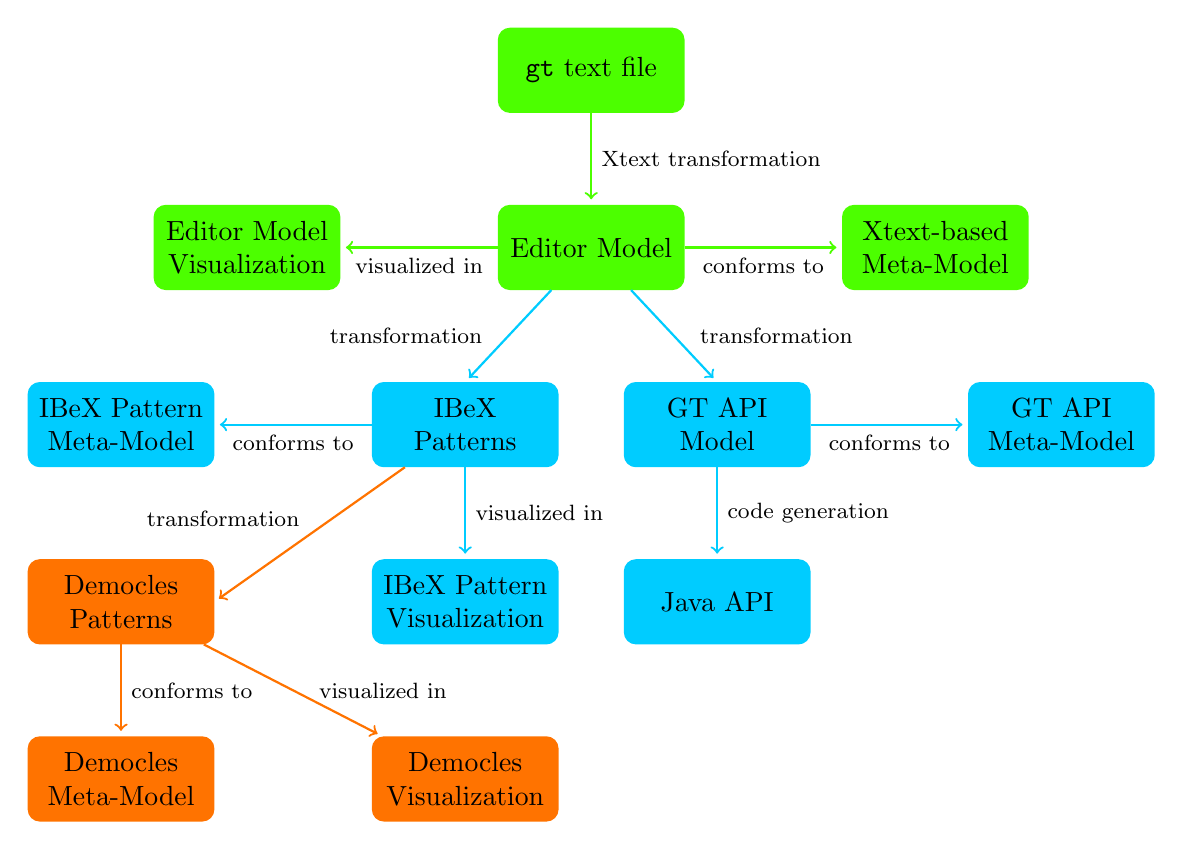
\begin{tikzpicture} [
		auto,
		node distance = 2.25cm,
		node/.style = {
			rectangle,
			rounded corners,
			thick,
			text width = 6em,
			text centered,
			minimum height = 3em,
		},
		line/.style = {
			draw,
			thick,
			->,
			shorten >=2pt,
		},
		line-caption/.style = {
			font = \footnotesize
		},
		ibex-ui/.style = {
			draw = green!60!lime,
			fill = green!60!lime,
		},
		ibex/.style = {
			draw = blue!20!cyan,
			fill = blue!20!cyan,
		},
		ibex-democles/.style = {
			draw = red!10!orange,
			fill = red!10!orange
		}
	]

	\node[node, ibex-ui] (f) {
		\texttt{gt} text file
	};

	\node[node, ibex-ui, below of = f] (e) {
		Editor Model
	};
	\node[node, ibex-ui, left = 2cm of e] (ev) {
		Editor Model Visualization
	};
	\node[node, ibex-ui, right = 2cm of e] (em) {
		Xtext-based Meta-Model
	};

	\node[node, ibex, below of = e, xshift = 1.6cm] (g) {
		GT API Model
	};
	\node[node, ibex, right = 2cm of g] (gm) {
		GT API Meta-Model
	};
	\node[node, ibex, below of = g] (gc) {
		Java API
	};

	\node[node, ibex, below of = e, xshift = -1.6cm] (i) {
		IBeX Patterns
	};
	\node[node, ibex, left = 2cm of i] (im) {
		IBeX Pattern Meta-Model
	};
	\node[node, ibex, below of = i] (iv) {
		IBeX Pattern Visualization
	};

	\node[node, ibex-democles, below of = im] (d) {
		Democles Patterns
	};
	\node[node, ibex-democles, below of = d] (dm) {
		Democles Meta-Model
	};
	\node[node, ibex-democles, below of = iv] (dv) {
		Democles Visualization
	};

	\begin{scope} [
			every path/.style = line, ibex-ui,
			every node/.style = line-caption
		]
		\path (f) -- node[right] {Xtext transformation} (e);
		\path (e) -- node[below] {visualized in} (ev);
		\path (e) -- node[below] {conforms to} (em);
	\end{scope}

	\begin{scope} [
			every path/.style = line, ibex,
			every node/.style = line-caption
		]
		\path (e) -- node[left, xshift = -0.2cm] {transformation} (i.north);
		\path (e) -- node[right, xshift = 0.2cm] {transformation} (g.north);

		\path (i) -- node[below] {conforms to} (im);
		\path (i) -- node[right] {visualized in} (iv);

		\path (g) -- node[below] {conforms to} (gm);
		\path (g) -- node[right] {code generation} (gc);
	\end{scope}

	\begin{scope} [
			every path/.style = line, ibex-democles,
			every node/.style = line-caption
		]
		\path (i) -- node[left, yshift = 0.2cm] {transformation} (d.east);
		\path (d) -- node[right] {conforms to} (dm);
		\path (d) -- node[right, xshift = 0.2cm] {visualized in} (dv);
	\end{scope}
\end{tikzpicture}

			}
		\end{center}
	\end{frame}

\subsection{Java API}
	\begin{frame}
		\frametitle{Graph Transformation with eMoflon::IBeX}
		\framesubtitle{Java API: Count Matches}
		\includegraphics[width=\textwidth]{../common/code/example-countMatches}
	\end{frame}
	\begin{frame}
		\frametitle{Graph Transformation with eMoflon::IBeX}
		\framesubtitle{Java API: Rule Application}
		\includegraphics[width=\textwidth]{../common/code/example-rule-application}
	\end{frame}
	\begin{frame}
		\frametitle{Graph Transformation with eMoflon::IBeX}
		\framesubtitle{Java API: Subscriptions -- Exploit Incrementality}
		\includegraphics[width=\textwidth]{../common/code/example-subscriptions}
	\end{frame}

\subsection{Integration with the TGG Part}
	\begin{frame}
		\frametitle{Graph Transformation with eMoflon::IBeX}
		\framesubtitle{Integration with the TGG Part}
		\begin{center}
			\resizebox{\linewidth}{!}{
				% !TeX encoding = UTF-8
% !TeX spellcheck = en_US

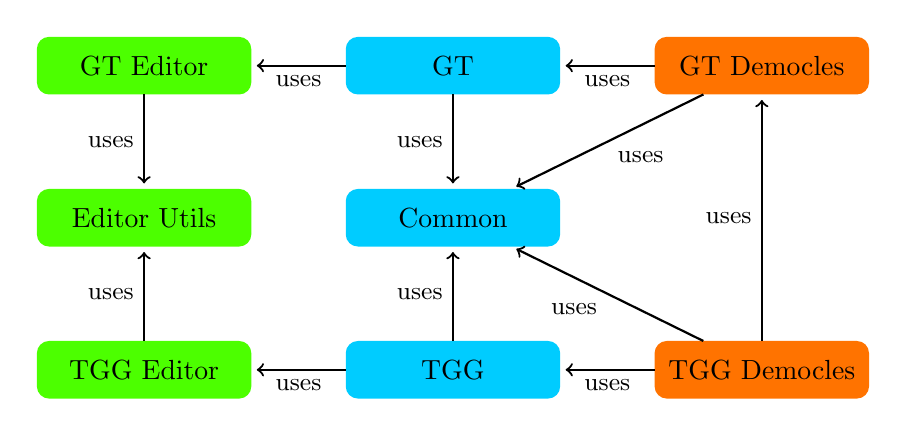
\begin{tikzpicture} [
		auto,
		node/.style = {
			rectangle,
			rounded corners,
			thick,
			text width = 7em,
			text centered,
			minimum height = 2em,
		},
		line/.style = {
			draw,
			thick,
			->,
			shorten >=2pt,
		},
		line-caption/.style = {
			font = \small,
		},
		ibex-ui/.style = {
			draw = green!60!lime,
			fill = green!60!lime,
		},
		ibex/.style = {
			draw = blue!20!cyan,
			fill = blue!20!cyan,
		},
		ibex-democles/.style = {
			draw = red!10!orange,
			fill = red!10!orange
		}
	]

	\matrix[
		column sep = 12mm,
		row sep = 12mm
	] {
		\node[node, ibex-ui] (uiGT) {
			GT Editor
		};
		& \node[node, ibex](GT) {
			GT
		};
		& \node[node, ibex-democles](democlesGT) {
			GT Democles
		};
		\\
		\node[node, ibex-ui] (uiCommon) {
			Editor Utils
		};
		& \node[node, ibex](common) {
			Common
		};
		\\
		\node[node, ibex-ui] (uiTGG) {
			TGG Editor
		};
		& \node[node, ibex](TGG) {
			TGG
		};
		& \node[node, ibex-democles](democlesTGG) {
			TGG Democles
		};
		\\
	};

	\begin{scope} [
		every path/.style = line,
		every node/.style = line-caption
		]
		\path (uiGT) -- node[left] {uses} (uiCommon);
		\path (uiTGG) -- node[left] {uses} (uiCommon);

		\path (GT) -- node {uses} (uiGT);
		\path (TGG) -- node {uses} (uiTGG);

		\path (GT) -- node[left] {uses} (common);
		\path (TGG) -- node[left] {uses} (common);

		\path (democlesGT) -- node {uses} (GT);
		\path (democlesGT) -- node {uses} (common);
		\path (democlesTGG) -- node {uses} (common);
		\path (democlesTGG) -- node {uses} (TGG);
		\path (democlesTGG) -- node {uses} (democlesGT);
	\end{scope}
\end{tikzpicture}

			}
		\end{center}
	\end{frame}

	% !TeX encoding = UTF-8
% !TeX spellcheck = en_US

\section{Evaluation and Future Work}
	\begin{frame}
		\frametitle{Contents}
		\tableofcontents[currentsection]
	\end{frame}
	\begin{frame}
		\frametitle{Evaluation and Future Work}
		\framesubtitle{Compliance with Requirements, JUnit Tests}
		\begin{itemize}
			\item Requirements fulfilled
				\begin{itemize}
					\item Application conditions only in DNF
					\item Limited set of attribute assignments and conditions
				\end{itemize}

			\only<2-3>{
			\item 2 JUnit test suites for 13 APIs with 90 test cases
				\begin{itemize}
					\item TestsuiteGT covers 90\,\% of the abstract classes and the interpreter
					\item Build of GT projects covers 94\,\% of the GT builder
					\item used in MBSE lecture (Summer Term 2018)
				\end{itemize}
			\item JUnit test suite for scoping/validation in the editor: 111 test cases, coverage 96\,\%
			}
		\end{itemize}
	\end{frame}
	\begin{frame}
		\frametitle{Evaluation and Future Work}
		\framesubtitle{End-User Survey: Textual Syntax and Visualization}
		\begin{center}
			\includegraphics[width=\linewidth]{../common/figures/evaluation-results-syntax}
		\end{center}
	\end{frame}
	\begin{frame}
		\frametitle{Evaluation and Future Work}
		\framesubtitle{End-User Survey: Java Integration}
		\begin{center}
			\includegraphics[width=.7\linewidth]{../common/figures/evaluation-results-java-integration}
		\end{center}
	\end{frame}
	\begin{frame}
		\frametitle{Evaluation and Future Work}
		\framesubtitle{Performance of Model Generation and Modification (linear time axis)}
		\begin{center}
			\includegraphics[height=.75\textheight]{../common/figures/evaluation-runtime1}
		\end{center}
	\end{frame}
	\begin{frame}
		\frametitle{Evaluation and Future Work}
		\framesubtitle{Performance of Model Generation and Modification (logarithmic time axis)}
		\begin{center}
			\includegraphics[height=.75\textheight]{../common/figures/evaluation-runtime1-logarithmic}
		\end{center}
	\end{frame}
	\begin{frame}
		\frametitle{Evaluation and Future Work}
		\framesubtitle{Performance of Model Queries (linear time axis)}
		\begin{center}
			\includegraphics[height=.75\textheight]{../common/figures/evaluation-runtime2}
		\end{center}
	\end{frame}
	\begin{frame}
		\frametitle{Evaluation and Future Work}
		\framesubtitle{Performance of Model Queries (logarithmic time axis)}
		\begin{center}
			\includegraphics[height=.75\textheight]{../common/figures/evaluation-runtime2-logarithmic}
		\end{center}
	\end{frame}
	\begin{frame}
		\frametitle{Evaluation and Future Work}
		\framesubtitle{Summary and Future Work}
		\begin{block}{eMoflon::IBeX-GT}
			\begin{itemize}
				\item Expressive pattern language with simple syntax
				\item Integration into Java via a generated, typed API
				\item Incremental features
				\item Shared libraries with eMoflon::IBeX-TGG
			\end{itemize}
		\end{block}

		\only<2>{
		\begin{block}{Future work}
			\begin{itemize}
				\item Evaluation of performance
				\item Optimization of the pattern network
				\item Shared IBeX patterns with TGG
			\end{itemize}
		\end{block}
		}
	\end{frame}

\end{document}
